% Svolgimento: prova del 17/07/2023, esercizio 1 (B72-E01) -- ugello aerospike piano in schlieren.
% Numeri e figure: calcoli.py (stessa cartella). Compilare con: latexmk -pdf svolgimento.tex

\documentclass[11pt,a4paper]{article}

\usepackage[T1]{fontenc}
\usepackage[utf8]{inputenc}
\usepackage[italian]{babel}
\usepackage{amsmath,amssymb}
\usepackage[a4paper,margin=2.5cm]{geometry}
\usepackage{array}
\usepackage{siunitx}
\usepackage{booktabs}
\usepackage{graphicx}
\usepackage{float}
\usepackage{caption}
\usepackage{hyperref}

\hypersetup{hidelinks}
\setlength{\parindent}{0pt}
\setlength{\parskip}{4pt}
\allowdisplaybreaks
\graphicspath{{figure/}}
\sisetup{output-decimal-marker={,}, group-separator={\,}, per-mode=symbol,
         exponent-product=\cdot, range-phrase={\text{--}}}

\newcommand{\Cp}{C^{+}}
\newcommand{\Cm}{C^{-}}

\title{Gasdinamica -- Prova del 17/07/2023, esercizio 1 (B72-E01)\\[2pt]
\large Ugello aerospike piano: lettura della schlieren}
\author{}
\date{}

\begin{document}
\maketitle

\section*{Traccia}
\emph{La fotografia schlieren mostra un flusso supersonico bidimensionale stazionario per un ugello aerospike. Il
rapporto di espansione (pressione totale / pressione esterna) è pari a 25. Descrivere il campo di flusso e
identificare le caratteristiche del flusso etichettate 1-2-3-4.} (10/30)

Traccia affine nel catalogo: B69-E03 (ugello a spina troncata in shadowgraph); per il progetto della spina ideale
B59-E02. Risolvo in modo indipendente.

%==============================================================================
\section{Lettura del testo e dell'immagine}
La schlieren rende visibili i gradienti di densità: urti e onde di Mach appaiono come linee nette e sottili, gli
strati di scorrimento come bande sfumate che si allargano. La luminosità dipende dal segno della componente del
gradiente normale al coltello, quindi strutture speculari nelle due metà possono avere tono opposto.

Si vede, attraverso una finestra circolare, un ugello \textbf{aerospike piano}: due feritoie, in alto e in basso,
ciascuna fra un \textbf{carenaggio} esterno (blocco nero con la faccia destra verticale) e la \textbf{spina} centrale,
che si assottiglia verso destra e termina con una piccola \textbf{base piana} (spina troncata). Il gas arriva dalla
camera a sinistra, attraversa le feritoie convergenti, che al \textbf{labbro} (spigolo del carenaggio) sono inclinate
verso l'asse, e scorre lungo la spina. La corrente va da sinistra verso destra e il campo è simmetrico rispetto
all'asse: studio la metà superiore, la inferiore è speculare ($\Cp\leftrightarrow\Cm$). Le strutture sono nitide e la
traccia dice che il moto è stazionario.

Dati: $p_0/p_a=25$. Non ci sono scale: riferisco le lunghezze a $h$, semidistanza fra i due labbri, e le pressioni
alla pressione ambiente $p_a$. Assumo aria, $\gamma=1{,}4$ (prova in galleria a freddo).

\begin{figure}[H]
  \centering
  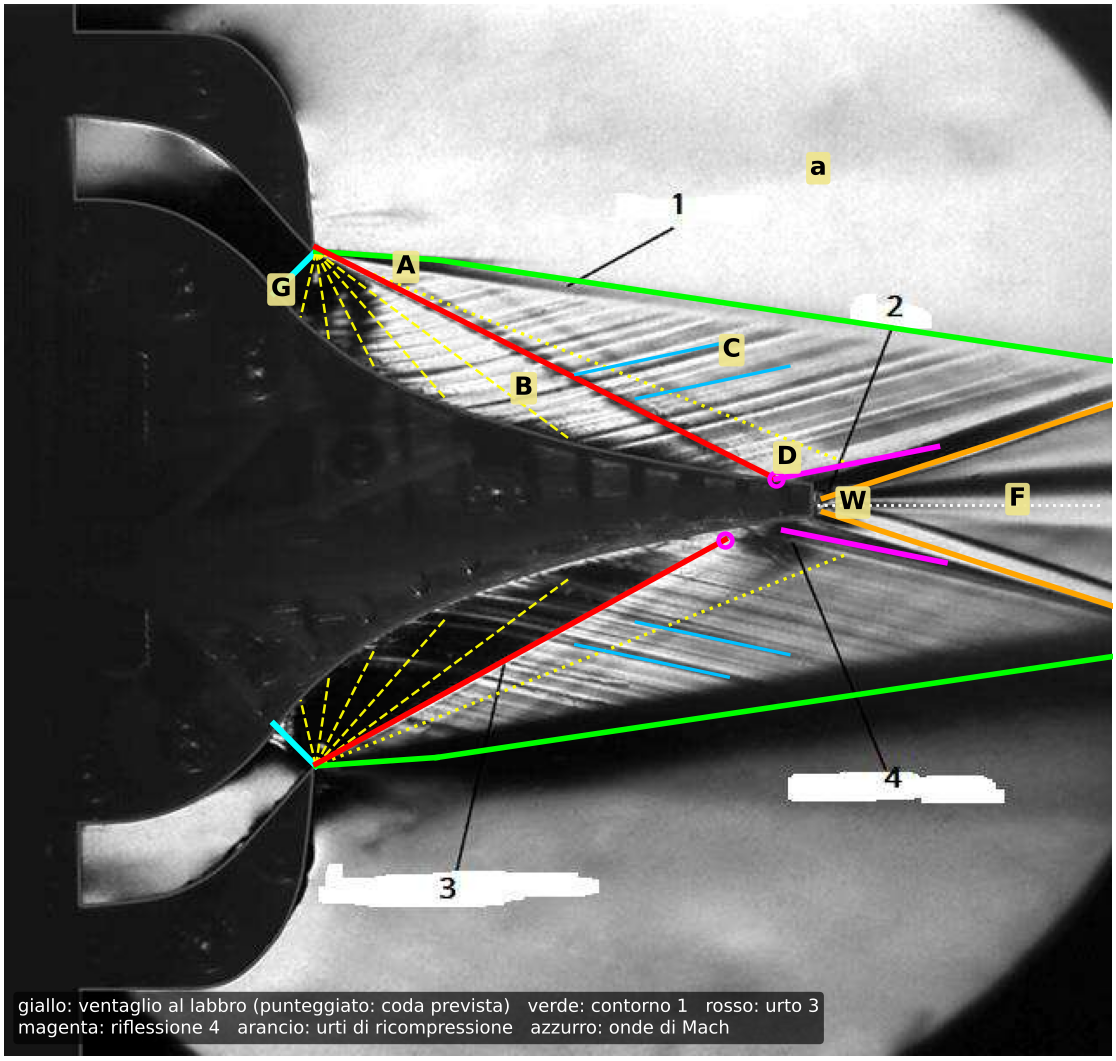
\includegraphics[width=0.80\textwidth]{annotata.png}
  \caption{Schlieren della traccia con le strutture identificate e gli stati (lettere). Ciano: gola G al labbro;
  giallo tratteggiato: raggi del ventaglio di Prandtl--Meyer centrato al labbro, punteggiato: dove ne cadrebbe la
  coda; verde: contorno del getto (1); rosso: urto 3; magenta: riflessione 4 sulla spina; arancio: urti di
  ricompressione della scia (2); azzurro: onde di Mach nella zona C. I numeri neri sono quelli della traccia.}
  \label{fig:ann}
\end{figure}

%==============================================================================
\section{Identificazione delle strutture}
Nell'ordine in cui le incontra la corrente (fig.~\ref{fig:ann}):
\begin{itemize}
\item \textbf{Gola G}, al labbro: le pareti della feritoia (carenaggio e spina) arrivano al labbro parallele,
  inclinate verso l'asse. Subito a valle compaiono linee di Mach: la corrente è già supersonica.
\item \textbf{Ventaglio di Prandtl--Meyer centrato al labbro} (non numerato): la corrente gira attorno allo spigolo
  del carenaggio ed espande verso la pressione ambiente; le sue onde, della famiglia $\Cm$, scendono verso la spina.
  È una regione, non una linea, e si riconosce dalle linee di Mach che vi cambiano inclinazione.
\item \textbf{1 -- Contorno del getto} (strato di taglio, \emph{shear layer}): separa il getto dall'aria ambiente in
  quiete. È una banda sfumata che si allarga verso valle perché vi avviene il mescolamento (contatto, linearmente
  degenere). Vi vale $p=p_a$; non è uno strato limite, perché non c'è parete. Parte quasi assiale dal labbro e poi si
  inclina verso l'asse.
\item \textbf{Linee sottili oblique dentro il getto}: onde di Mach deboli della famiglia $\Cp$ (nella metà inferiore
  $\Cm$), generate dalle piccole irregolarità della spina. Che si vedano caratteristiche di entrambe le famiglie dice
  che il campo lungo la spina \textbf{non è un'onda semplice}.
\item \textbf{3 -- Urto obliquo debole}: linea netta e rettilinea che parte dalla zona del labbro e attraversa il getto
  fino alla spina. Le espansioni che arrivano dal lato della spina raggiungono il contorno libero e si riflettono con
  natura opposta, cioè come compressioni $\Cm$; queste convergono e si raccolgono in un urto. Non è la coda del
  ventaglio del labbro: la sua inclinazione è diversa da quella della coda (calcolo, punto c).
\item \textbf{4 -- Riflessione di 3 sulla spina}, poco a monte della troncatura: su una parete l'urto si riflette con
  la stessa natura, quindi da lì riparte un urto (famiglia $\Cp$ in alto, $\Cm$ in basso) verso il contorno. Vicino
  alla parete la riflessione occupa una piccola zona scura: è l'interazione con lo strato limite della spina.
\item \textbf{2 -- Scia della base troncata}: la corrente gira attorno agli spigoli della base con un'espansione di
  Prandtl--Meyer, dietro la base c'è una piccola zona di ricircolo W (``poppa fluida''), e dove i due getti si
  incontrano due \textbf{urti di ricompressione} li riallineano all'asse. Più a valle si vede la scia lungo l'asse.
\end{itemize}
Non sono strutture del campo i riquadri bianchi dei numeri, il bordo della finestra e il fondo, più chiaro sopra e più
scuro sotto per l'illuminazione non uniforme.

%==============================================================================
\section{Modello e ipotesi}
\begin{itemize}
\item \textbf{Gola sonica al labbro.} Le feritoie sono convergenti e terminano al labbro con pareti parallele; subito a
  valle si vedono linee di Mach. Quindi la gola è efficace e $M=1$ al labbro, con la direzione delle pareti,
  $\theta_0$.
\item \textbf{2D stazionario supersonico} nel getto: linee di Mach si vedono ovunque fra la spina e il contorno, quindi
  tutte le regioni del getto sono supersoniche. Il modello non vale nella zona di ricircolo W, subsonica, né dentro lo
  strato di taglio.
\item \textbf{Contorno libero}: sul contorno del getto $p=p_a$; l'aria esterna è in quiete. Sulla spina la corrente è
  tangente alla parete.
\item \textbf{Isentropico fuori dagli urti}, con $p_0$ uniforme in camera. Gli urti visibili sono sottili e quasi
  inclinati come le onde di Mach, quindi deboli: tratto $p_0$ come costante nel getto e lo verifico a posteriori.
  Ne segue che \textbf{sul contorno, dove $p=p_a$, il numero di Mach è lo stesso ovunque}, $M_a$.
\item Le onde di Mach sono rettilinee nelle zone uniformi; nel ventaglio e nella zona d'interazione lungo la spina
  sono curve. Le misure di direzione le faccio nelle zone uniformi.
\end{itemize}

%==============================================================================
\section{Misure sull'immagine}
Con righello e goniometro, prendendo l'asse come la mezzeria fra i due labbri e la base (angoli antiorari
dall'asse; i valori sono quelli della metà superiore, e la metà inferiore dà gli stessi valori con segno opposto):
\begin{table}[H]
  \centering
  \begin{tabular}{lc}
    \toprule
    Grandezza & Valore misurato \\
    \midrule
    pareti della feritoia al labbro (direzione della corrente in gola) & $\theta_0\approx\ang{-45}$ \\
    contorno 1, primo tratto (fino a circa $0{,}5\,h$) & $\approx\ang{-4}$ \\
    contorno 1, a valle & $\theta_C\approx\ang{-8.5}$ \\
    urto 3 & $\approx\ang{-28}$ \\
    onde di Mach fra 3 e 1 (zona C) & $\approx\ang{12}$ \\
    ultimo tratto della spina & $\approx\ang{-9}$ \\
    retta dal labbro allo spigolo della base & $\approx\ang{-25}$ \\
    urto riflesso 4 & $\approx\ang{12}$ \\
    urti di ricompressione della scia & $\approx\pm\ang{18}$ \\
    \midrule
    punto di riflessione R di 3 sulla spina & $x_R\approx1{,}7\,h$ dal labbro \\
    base della spina & $x\approx1{,}95\,h$, altezza $\approx0{,}13\,h$ \\
    \bottomrule
  \end{tabular}
\end{table}

%==============================================================================
\section{Analisi qualitativa}
\begin{itemize}
\item In gola $p^*=0{,}528\,p_0$, molto più della pressione ambiente: il getto in uscita dalle feritoie è fortemente
  \textbf{sottoespanso} e il resto dell'espansione avviene fuori, a valle del labbro. È il principio
  dell'aerospike: dal lato esterno non c'è parete ma il contorno libero a $p=p_a$, quindi il getto si adatta da sé
  alla pressione ambiente.
\item Al labbro la corrente gira attorno allo spigolo con un \textbf{ventaglio di Prandtl--Meyer centrato} (onde
  $\Cm$): espande fino a $p_a$ e ruota verso la direzione assiale. Le onde del ventaglio scendono verso la spina.
\item Una \textbf{spina ideale} è la linea di corrente dell'onda semplice: la parete ruota punto per punto come la
  corrente, quindi le onde che vi arrivano non si riflettono e il getto esce uniforme e assiale. La spina reale è
  troncata e non segue esattamente quella linea di corrente: dove ruota meno di quanto richiede l'onda semplice
  manda nel getto \textbf{espansioni} $\Cp$.
\item Le espansioni raggiungono il contorno libero, lo piegano verso l'asse e si riflettono, a pressione costante, con
  natura opposta: \textbf{compressioni} $\Cm$. Le compressioni convergono e formano l'urto debole \textbf{3}, che
  attraversa il getto e si riflette sulla spina (\textbf{4}) come urto, cioè con la stessa natura.
\item Alla troncatura i getti superiore e inferiore, inclinati verso l'asse, girano attorno agli spigoli della base
  (espansioni), racchiudono la zona di ricircolo W, a pressione minore di $p_a$, e si incontrano a valle, dove gli
  \textbf{urti di ricompressione} li riportano paralleli all'asse (\textbf{2}).
\end{itemize}

%==============================================================================
\section{Topologia del campo}
\begin{figure}[H]
  \centering
  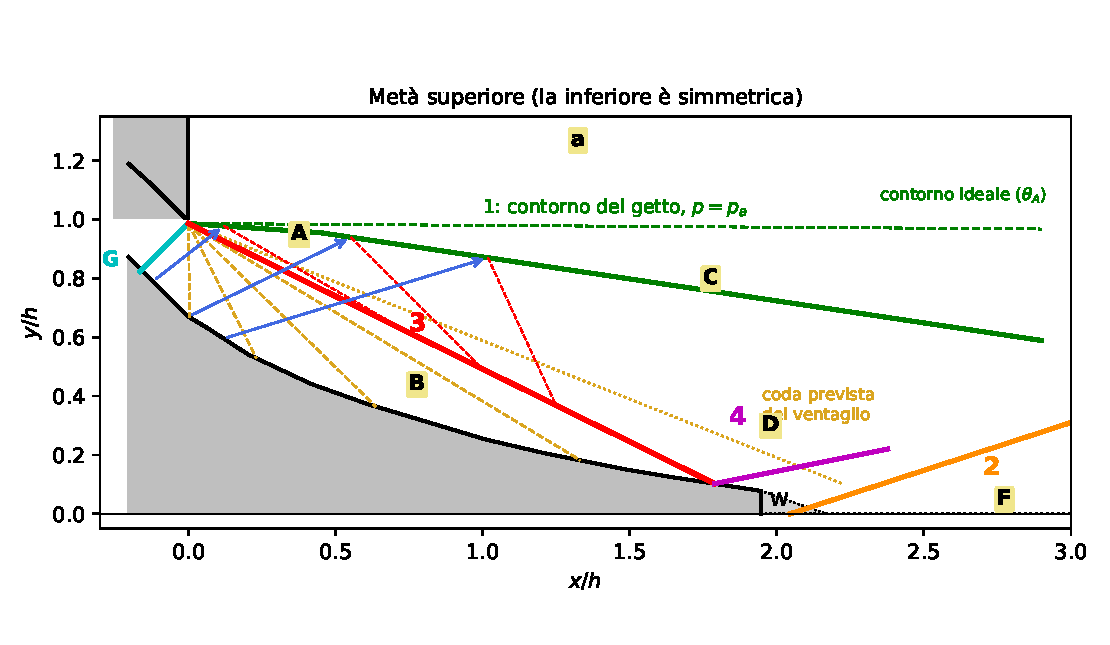
\includegraphics[width=0.88\textwidth]{schema.pdf}
  \caption{Schema della metà superiore in unità di $h$, con la spina e i labbri misurati: gola G (ciano), raggi del
  ventaglio al labbro e coda prevista (ocra), espansioni dal lato della spina (blu) che si riflettono sul contorno
  come compressioni (rosso tratteggiato) convergenti nell'urto 3, riflessione 4, zona di ricircolo W, urto di
  ricompressione 2 e scia sull'asse.}
  \label{fig:schema}
\end{figure}

\begin{table}[H]
  \centering
  \small
  \begin{tabular}{cp{6.6cm}p{5.4cm}}
    \toprule
    Stato & Dove & Come lo si raggiunge \\
    \midrule
    a & aria ambiente in quiete, $p=p_a$ & -- \\
    G & gola al labbro: $M=1$, $\theta=\theta_0$ & convergente \\
    A & a valle del ventaglio, lungo il contorno vicino al labbro: $p=p_a$ & ventaglio $\Cm$ centrato al labbro \\
    B & fra la spina e 3: zona a due famiglie (non onda semplice); stato rappresentativo davanti a 3 & espansioni
    $\Cp$ dal lato della spina \\
    C & fra 3 e il contorno 1, a valle: $p\simeq p_a$ & urto 3 ($\Cm$) \\
    D & dietro la riflessione 4, lungo l'ultimo tratto della spina & urto riflesso 4 ($\Cp$) \\
    W & zona di ricircolo dietro la base, subsonica, $p_W<p_a$ & espansione agli spigoli della base \\
    F & a valle della scia, corrente assiale & urto di ricompressione ($\Cp$) \\
    \bottomrule
  \end{tabular}
  \caption{Stati della metà superiore. Fra 1 e l'aria ambiente c'è lo strato di taglio.}
\end{table}
La zona B, dove sono attive entrambe le famiglie, si potrebbe risolvere con il metodo delle caratteristiche
(compatibilità lungo $\Cp$ e $\Cm$ più la condizione di parete), ma la soluzione non è analitica e non serve per
riconoscere le strutture: ne uso solo uno stato rappresentativo.

%==============================================================================
\section{Calcolo}

\subsection*{a) Gola e grado di sottoespansione}
\[
\frac{p^*}{p_0}=\Big(\frac{2}{\gamma+1}\Big)^{\frac{\gamma}{\gamma-1}}=0{,}528
\qquad\Rightarrow\qquad \frac{p_G}{p_a}=\frac{p_0}{p_a}\,\frac{p^*}{p_0}=13{,}2 .
\]

\subsection*{b) Stato sul contorno del getto}
Sul contorno $p=p_a$ e $p_0$ è quello di camera:
\[
\frac{p_0}{p_a}=\big(1+\delta M_a^2\big)^{\frac{\gamma}{\gamma-1}}\ \Rightarrow\ M_a=2{,}75,\qquad
\nu_a=\nu(M_a)=\ang{44.6},\qquad \mu_a=\arcsin\frac1{M_a}=\ang{21.4}.
\]

\subsection*{c) Ventaglio al labbro: stato A e coda del ventaglio}
Le onde del ventaglio sono $\Cm$; attraversandole ci si muove lungo una $\Cp$, su cui si conserva $\theta-\nu$. Dalla
gola ($\nu=0$, $\theta=\theta_0$) al contorno ($\nu=\nu_a$):
\[
\theta_A-\nu_a=\theta_0-0\qquad\Rightarrow\qquad \theta_A=\theta_0+\nu_a\approx\ang{-0.4}\approx0 .
\]
Le feritoie sono inclinate proprio di $\nu(M_a)$: è la condizione di progetto della spina ideale ($|\theta_0|=\nu(M_e)$),
per cui il solo ventaglio porterebbe la corrente a $p_a$ e in direzione assiale. L'ultima onda del ventaglio è la $\Cm$
dello stato A:
\[
\theta_{\rm coda}=\theta_A-\mu_a\approx\ang{-21.7},
\]
e raggiungerebbe l'asse a $x=h/\tan\mu_a\approx2{,}56\,h$: la spina reale, lunga $1{,}95\,h$, è troncata a circa tre
quarti. La linea 3 è inclinata di circa \ang{-28}, sei gradi più della coda: \textbf{3 non è la coda del ventaglio}.

\subsection*{d) Contorno piegato verso l'asse: ampiezza delle espansioni}
Il contorno lascia il labbro quasi nella direzione $\theta_A$ e a valle è inclinato di $\theta_C\approx\ang{-8.5}$.
Un'espansione $\Cp$ di ampiezza $\Delta\nu$ che arriva sul contorno: attraversandola si va lungo una $\Cm$, dove
$\theta+\nu$ è costante, quindi $\theta$ cala di $\Delta\nu$. La riflessa $\Cm$ riporta $p$ a $p_a$, cioè $\nu$ a
$\nu_a$; attraversandola si va lungo una $\Cp$, dove $\theta-\nu$ è costante, quindi $\theta$ cala di altri
$\Delta\nu$. In tutto il contorno ruota di $2\Delta\nu$:
\[
\Delta\nu=\frac{\theta_A-\theta_C}{2}\approx\ang{4.1}.
\]

\subsection*{e) Stato B, davanti all'urto 3}
È lo stato vicino al contorno raggiunto dalle espansioni e non ancora dalle compressioni riflesse:
\begin{gather*}
\nu_B=\nu_a+\Delta\nu\approx\ang{48.7}\ \Rightarrow\ M_B\approx2{,}94,\qquad
\theta_B=\theta_A-\Delta\nu\approx\ang{-4.4},\\
\frac{p_B}{p_a}=\frac{p_0}{p_a}\big(1+\delta M_B^2\big)^{-\frac{\gamma}{\gamma-1}}\approx0{,}74 .
\end{gather*}
In B il getto è localmente sovraespanso.

\subsection*{f) Urto 3}
Le compressioni riflesse riportano la corrente a $p_a$ e la ruotano di altri $\Delta\nu$: raccolte nell'urto 3 (famiglia
$\Cm$), questo devia la corrente di $\theta=\Delta\nu$ a partire da B. Con la relazione $\theta$--$\sigma$--$M$, che
viene dalle relazioni di salto applicate alla componente normale ($M_{n1}=M_B\sin\sigma$) con la tangenziale
conservata,
\[
\tan\theta=2\cot\sigma\,\frac{M_B^2\sin^2\sigma-1}{M_B^2(\gamma+\cos2\sigma)+2}
\quad\Rightarrow\quad \sigma\approx\ang{22.8},\qquad M_{n1}=M_B\sin\sigma\approx1{,}14,
\]
\[
\frac{p_C}{p_B}=1+\frac{2\gamma}{\gamma+1}\big(M_{n1}^2-1\big)\approx1{,}35
\quad\Rightarrow\quad p_C\approx p_a,\qquad M_C\approx2{,}75,\qquad \frac{p_{0C}}{p_{0B}}\approx0{,}997 .
\]
Il fronte dell'urto è inclinato di
\[
\theta_B-\sigma\approx\ang{-27.2},
\]
contro \ang{-28} misurati: la linea 3 è proprio l'urto formato dalle compressioni riflesse.

\subsection*{g) Mach nella zona C dalle onde di Mach}
Nella zona C le onde $\Cp$ sono rettilinee e inclinate di $\theta_C+\mu_C$; con le due inclinazioni misurate:
\[
\mu_C=\phi_{\Cp}-\theta_C\approx\ang{20.5}\quad\Rightarrow\quad M_C=\frac1{\sin\mu_C}\approx2{,}9 ,
\]
vicino a $M_a=2{,}75$ (in C $p\simeq p_a$). Per $M$ elevati $\mu$ varia poco con $M$, quindi questo valore è solo
indicativo.

\subsection*{h) La spina non è la linea di corrente dell'onda semplice}
Sia $\phi_R\approx\ang{-25}$ l'inclinazione della retta che va dal labbro allo spigolo della base. Se il campo fosse
il solo ventaglio centrato, questa retta sarebbe una delle sue onde $\Cm$: $\theta-\mu=\phi_R$, con
$\theta=\theta_0+\nu$, cioè
\[
\nu(M)-\mu(M)=\phi_R-\theta_0\quad\Rightarrow\quad M\approx2{,}64,\qquad
\theta_{\rm ideale}=\theta_0+\nu(M)\approx\ang{-2.7}.
\]
L'ultimo tratto della spina è invece inclinato di circa \ang{-9}: la parete ruota circa \ang{6} meno di quanto
richiede l'onda semplice, quindi genera espansioni $\Cp$ di qualche grado, dello stesso ordine del $\Delta\nu\approx\ang{4}$
ricavato dal contorno.

\subsection*{i) Riflessione 4}
La deviazione dell'urto incidente, $\approx\ang{4}$, è molto minore dell'angolo di distacco
$\theta_D(M_B)\approx\ang{21}$: la riflessione è \textbf{regolare}, come si vede (nessun gambetto di Mach). Stima con la
corrente lungo l'ultimo tratto della spina ($\theta_w=\ang{-9}$, $M\simeq M_B$): l'incidente devia di $-\Delta\nu$ con
$\sigma\approx\ang{22.8}$; il riflesso ($\Cp$) riporta la corrente parallela alla parete con $\sigma_r\approx\ang{24.4}$,
quindi il suo fronte è inclinato di
\[
\theta_w-\Delta\nu+\sigma_r\approx\ang{11},\qquad \frac{p_D}{p_a}\approx1{,}3 ,
\]
contro circa \ang{12} misurati.

\subsection*{l) Scia della base (2)}
Nella zona di ricircolo W la corrente è subsonica e il modello 2D supersonico non vale: so solo che $p_W<p_a$ (la
corrente vi entra espandendo attorno agli spigoli della base). Stimo la ricompressione con un solo urto $\Cp$ che
riporta all'asse il getto della zona C ($M_a$, $\theta_C$), con deviazione $|\theta_C|$:
\[
\sigma\approx\ang{28.0},\qquad \text{fronte a }\theta_C+\sigma\approx\ang{19.5},\qquad
\frac{p_F}{p_a}\approx1{,}8,\qquad M_F\approx2{,}36 ,
\]
contro circa \ang{18} misurati. La stima ignora l'espansione agli spigoli della base, che prima abbassa la pressione e
aumenta la deviazione da recuperare.

%==============================================================================
\section{Verifiche a posteriori}
\begin{enumerate}
\item Direzione della gola: $|\theta_0|\approx\ang{45}$ misurato contro $\nu(M_a)=\ang{44.6}$. \emph{Coerente con un
  ugello di progetto per $p_0/p_a=25$.}
\item Urto 3: $M_{n1}\approx1{,}14>1$, $\Delta s>0$; deviazione \ang{4.1} $<\theta_{\max}(M_B)=\ang{33.7}$ e
  $\sigma=\ang{22.8}$ minore dell'angolo del punto di $\theta_{\max}$ (\ang{65}): ramo debole. Perdita di pressione
  totale dello 0,3\,\%. \emph{Verificata: urto debole, quasi isentropico.}
\item Condizione sul contorno: dietro 3 $p_C\approx p_a$. \emph{Verificata.}
\item Inclinazione di 3: \ang{-27.2} calcolata contro \ang{-28} misurata; la coda del ventaglio sarebbe a
  \ang{-21.7}. \emph{Verificata: 3 è l'urto delle compressioni riflesse.}
\item Mach in C dalle onde di Mach: $\approx2{,}9$ contro $M_a=2{,}75$. \emph{Coerente.}
\item Riflessione 4: deviazione $\approx\ang{4}\ll\theta_D\approx\ang{21}$, fronte \ang{11} contro \ang{12}.
  \emph{Verificata: riflessione regolare.}
\item Ricompressione: deviazione \ang{8.5} $<\theta_{\max}(M_a)=\ang{32.1}$, ramo debole, fronte \ang{19.5} contro
  \ang{18}. \emph{Coerente.}
\item Regioni del getto supersoniche: $M$ fra 1 (G) e 2,94 (B), $M_C\approx2{,}75$, $M_D\approx2{,}56$,
  $M_F\approx2{,}36$. \emph{Verificata}; resta esclusa la zona di ricircolo W, dove il modello non si applica.
\end{enumerate}

%==============================================================================
\section{Risultati}
\begin{table}[H]
  \centering
  \small
  \begin{tabular}{cp{6.8cm}p{5.6cm}}
    \toprule
    & Struttura & Valori \\
    \midrule
    1 & contorno del getto: strato di taglio fra getto e aria in quiete, $p=p_a$ & $M=M_a=2{,}75$; inclinazione da
    $\approx0$ a $\approx\ang{-8.5}$ \\
    2 & scia della base troncata: espansioni agli spigoli, ricircolo W ($p_W<p_a$), urti di ricompressione, scia
    sull'asse & urti a $\approx\pm\ang{18}$; $p_F\approx1{,}8\,p_a$ \\
    3 & urto obliquo debole formato dalle compressioni in cui le espansioni del lato spina si riflettono sul contorno
    libero & $\sigma\approx\ang{23}$, $M_{n1}\approx1{,}14$, $p_C/p_B\approx1{,}35$ \\
    4 & riflessione regolare di 3 sulla spina, poco a monte della base & riflesso a $\approx\ang{12}$,
    $p_D\approx1{,}3\,p_a$ \\
    \midrule
    & gola al labbro & $M=1$, $\theta_0\approx\ang{-45}$, $p^*=13{,}2\,p_a$ \\
    & stato adattato sul contorno & $M_a=2{,}75$, $\nu_a=\ang{44.6}$, $\mu_a=\ang{21.4}$ \\
    \bottomrule
  \end{tabular}
\end{table}
$M_a$, $\nu_a$, $\mu_a$ e $p^*/p_a$ sono esatti per i dati; gli altri valori dipendono dagli angoli misurati e sono
stime.

%==============================================================================
\section{Rappresentazioni}
\begin{figure}[H]
  \centering
  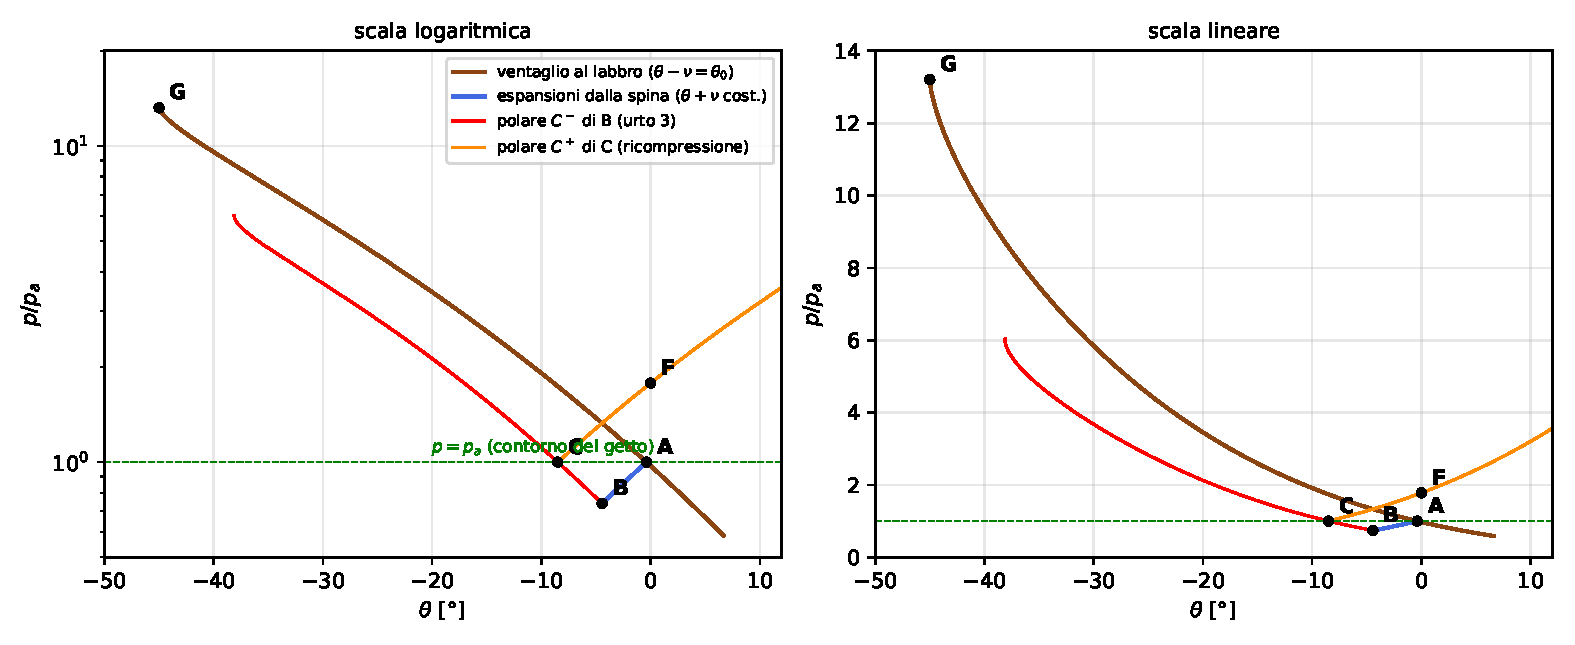
\includegraphics[width=\textwidth]{p_theta.pdf}
  \caption{Piano $p$--$\theta$ della metà superiore, in scala logaritmica e lineare: ventaglio al labbro
  ($\theta-\nu=\theta_0$, marrone), espansioni dal lato della spina (blu), polare $\Cm$ di B (urto 3, rosso) e polare
  $\Cp$ di C (ricompressione, arancio).}
  \label{fig:pth}
\end{figure}
\begin{figure}[H]
  \centering
  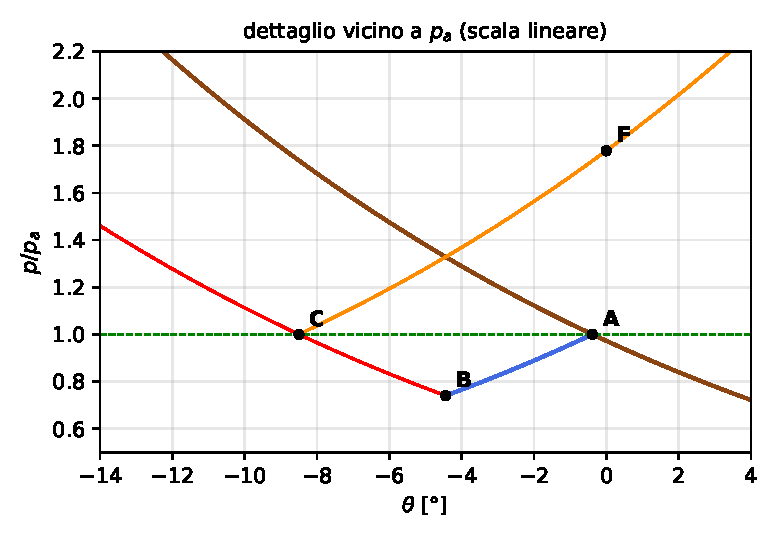
\includegraphics[width=0.58\textwidth]{p_theta_dettaglio.pdf}
  \caption{Dettaglio del piano $p$--$\theta$ vicino a $p_a$ (scala lineare).}
  \label{fig:pthd}
\end{figure}
\textbf{Piano $p$--$\theta$} (fig.~\ref{fig:pth}--\ref{fig:pthd}). Le pressioni vanno da $13{,}2\,p_a$ in gola a
$0{,}74\,p_a$ in B, più di un ordine di grandezza, quindi riporto entrambe le scale. Nella scala logaritmica si vede
tutto il percorso: dalla gola G il ventaglio al labbro scende lungo la curva $\theta-\nu=\theta_0$ e taglia la retta
$p=p_a$ in A, quasi a $\theta=0$; con una pressione ambiente più bassa la curva proseguirebbe oltre A e il contorno ruoterebbe verso
l'esterno. Nella scala lineare si vede che quasi tutta la caduta di pressione
avviene nel ventaglio, e che le onde successive sono piccole perturbazioni attorno a $p_a$. Il dettaglio mostra il
ciclo vicino a $p_a$: da A le espansioni del lato spina (blu, $\theta+\nu$ costante) portano a B, sotto $p_a$; la polare
$\Cm$ di B (urto 3) torna sulla retta $p=p_a$ in C, con $\theta_C$ uguale all'inclinazione misurata del contorno.
Infine la polare $\Cp$ di C, percorsa verso $\theta=0$, dà lo stato F dietro la ricompressione della scia.

Lo schema (fig.~\ref{fig:schema}) e l'immagine annotata (fig.~\ref{fig:ann}) riportano la stessa topologia: la
coda prevista del ventaglio (punteggiato) cade sensibilmente sopra la linea 3, mentre i fronti calcolati di 3, 4 e
della ricompressione coincidono con le linee visibili.

%==============================================================================
\section{Coerenza con l'immagine e discussione}
\begin{itemize}
\item \textbf{Autoadattamento.} Con le feritoie inclinate di $\nu(M_a)$ l'ugello lavora vicino al progetto: il getto
  esce quasi assiale e nel campo ci sono solo onde deboli ($\Delta\nu\approx\ang{4}$, urto 3 con $M_{n1}\approx1{,}14$).
  È il vantaggio dell'aerospike: il lato esterno è il contorno libero a $p=p_a$, quindi a pressioni ambiente diverse
  il getto cambia forma senza gli urti forti e le separazioni di un ugello a campana fuori progetto.
\item \textbf{Il campo non è un'onda semplice.} Le linee di Mach della famiglia $\Cp$ che attraversano il getto, il
  contorno che si piega verso l'asse e l'urto 3 dicono la stessa cosa: la spina non assorbe del tutto il ventaglio,
  perché è troncata e il suo profilo ruota meno della linea di corrente dell'onda semplice. Le misure (contorno,
  spina, inclinazione di 3) danno tutte espansioni di qualche grado, coerenti fra loro.
\item \textbf{Troncatura.} Tagliare la spina a circa tre quarti della lunghezza ideale fa completare una parte
  dell'espansione nella scia: la base vede una pressione $p_W<p_a$, quindi una resistenza di base, e i due getti si
  ricomprimono con urti. È il prezzo di una spina più corta e leggera.
\item \textbf{Limiti.} La zona di ricircolo è subsonica e richiede un modello diverso; lo strato di taglio e lo strato
  limite della spina sono viscosi (la riflessione 4 è allargata dall'interazione con lo strato limite); le pareti
  laterali della galleria introducono effetti tridimensionali. Le stime dipendono da angoli di pochi gradi: per
  esempio $M_C$ dall'angolo di Mach è solo indicativo.
\item Nella metà inferiore si vedono le stesse strutture speculari (3 e 4 sono indicate lì nella traccia); il tono
  diverso delle stesse strutture nelle due metà è un effetto del coltello, non del campo.
\end{itemize}

\end{document}
